\chapter{Analysis}

%\textit{Note: This chapter follows the Requirements Analysis Document Template in \cite{bruegge2004object}. 
%\textbf{Important:} Make sure that the whole chapter is independent of the chosen technology and development platform. The idea is %that you illustrate concepts, taxonomies and relationships of the application domain independent of the solution domain!
%Cite \cite{bruegge2004object} several times in this chapter.}

The analysis process results in a model of the system that aims to be correct, complete, consistent and unambiguous \cite{bruegge2004object}. In this chapter, we focus on scenario-based analysis. Firstly, we identify the functional and nonfunctional requiremens of the system. We subsequently design a use case model that depicts the different interactions between the users and the system. Furthermore, we identify and study the objects of our system.

\section{Requirements}
A requirement is a feature that the system must have or a constraint that it must satisfy to be accepted by the client \cite{bruegge2004object}. Requirements elicitation requires domain knowledge of the problem statement as well as experience in building software systems. In this section we elicit the functional and nonfunctional requirements of our system.

\subsection{Functional Requirements}

Functional requirements (FRs) describe the interactions between the system and the its environment independent of its implementation \cite{bruegge2004object}.

The system's main function is to classify images of different small parts. Furthermore, the system needs to be dynamic and scalable to accomodate new small parts. To ensure that the system is able to classify images accurately, while leveraging synthetic input images, we introduce the following Functional Requirements.

\begin{itemize}
  \item [FR1] \textbf{Generate Synthetic Images}: Given a 3D model of a small part, the system should generate a set of synthetic images of the model. The system should apply random rotation and translation to the 3D model before rendering the 2D synthetic image to ensure that the generated dataset captures the small part from different angles, and in different positions.

  \item [FR2] \textbf{Add New Class to the Classification Model}: The system should accomodate the addition of a new small part to the model. The system should be able to label new output classes.

  \item [FR3] \textbf{Adjust Input Data Split}: The system should allow for changes in the training, validation and testing input data which is assigned as input to the model. This includes changing the number of images in each set and manipulating the ratio of synthetic to real images in the training split.

  \item [FR4] \textbf{Retrain Classification Model}: The system should be able to retrain the classification model. This step is usually taken after the augmentation or adjustment of the input data split.

  \item [FR5] \textbf{Fine-Tune Classification Model}: The underlying CNN algorithm should be subject to fine-tuning in order to maximize the accuracy of the system.
\end{itemize}

\subsection{Nonfunctional Requirements}

Nonfunctional Requirements (NFRs) are key system requirements that apply to the system as a whole \cite{bruegge2004object}. To maintain the system's general requirements we define the following nonfunctional requirements.

\begin{itemize}
  \item [NFR1] \textbf{Performance}: A performence requirement is the measure of a quantifiable attribute of our system. In our case we would like to track our system's \textbf{classification accuracy}.\\
  We first define our system's accuracy for a single class to be the percentage of the given class's testing image split that the image classifier correctly predicts. We consequently define our system's classification accuracy to be the image classifier's average prediction accuracy over each class.

  \item [NFR2] \textbf{Adaptability}: Adaptability is the ability to change the system to deal with additional application domain concepts \cite{bruegge2004object}. Our system needs to be dynamic enough to accomodate for new small parts that can be later added even after the system has been deployed.
\end{itemize}

\section{System Models}
In this section we take a closer look at the system models. We identify the objects of our system, we examine their behaviour and we study the relationship between them. Moreover, we examine the use cases and activities of our system.

\subsection{Use Case Model}

Use case models represent the relationship between the user group of a system and the general functions that they can execute. A use case model can reduce the complexity of a system and increase its understandability.

The use case model of our system can be found as figure [\ref{fig:UCM}]. The two main protagonists of our system are the data generator, who is tasked with generating synthetic and real images, and the machine learning expert, who is responsible for training the system to classify a set of small parts.

\begin{figure}[H]
\centering
  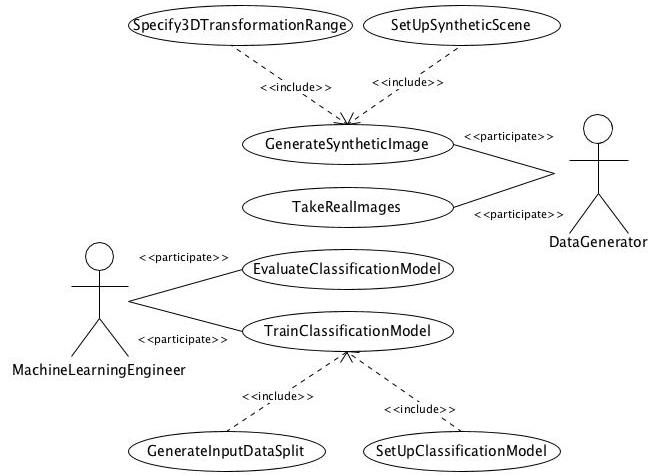
\includegraphics[width=\textwidth]{UCM}
\caption{Use Case Model}
\label{fig:UCM}
\end{figure}

The use case model can be divided into 3 main functions; namely generating synthetic images, obtaining real images, and training an image classifier.

\subsubsection{Generating Synthetic Images}

Generating synthetic images the cornerstone for a synthetically augmented dataset. There's a lot of work that goes into generating the 3D synthetic scene and the corresponding renditions. To increase the understandability of our model, we have separated the the use case that revolve around modeling the small part 3D model itself as \textit{Specify3DTransformations}, and the use case that deals with the synthetic scene environment as \textit{SetUpSyntheticScene}.

\begin{usecase}
  \addtitle{Use Case}{Specify3DTransformations}

  \addfield{Participating Actors}{DataGenerator}

  \addscenario{Flow of Events}{
    \item In the modeling software, the DataGenerator chooses the transformations that are applicable to the small part's 3D model.
    \item For each transformation, the DataGenerator sets the range of each tranformation attribute that will be later used to generate a random position for the synthetic image of the small part.
  }

  \additemizedfield{Entry Condition}{
    \item DataGenerator has modeling software open.
  }

  \additemizedfield{Exit Condition}{
    \item All the desired transformations and their corresponding attributes have been specified.
  }

  \additemizedfield{Quality Requirements}{
    \item In the effort to achieve the Performance Nonfunctional requirement, synthetic images have to look as photo realistic as possible. The 3D transformations should strive to output the range of positions that the respective small part can be placed in.
  }
\end{usecase}

\clearpage
\begin{usecase}
  \addtitle{Use Case}{SetUpSyntheticScene}

  \addfield{Participating Actors}{DataGenerator}

  \addscenario{Flow of Events}{
    \item In the modeling software, the DataGenerator places the 3D model of the small part on a horizontal plane as if lying on a table.
    \item The DataGenerator sets the background of the horizontal plane to mimic the background of the real images in the dataset.
    \item The DataGenerator sets the lighting condition of the scene to reflect the lighting condition of the environment where the real small part images are taken.
  }

  \additemizedfield{Entry Condition}{
    \item DataGenerator has modeling software open.
  }

  \additemizedfield{Exit Condition}{
    \item In the modeling software, the 3D model of the small part should be lying on a horizontal plane.
    \item The background and lighting condition should reflect the environment of the real small part images.
  }

  \additemizedfield{Quality Requirements}{
    \item The synthetic scene should look as photorealistic as possible. This helps the Image Classifier achieve a higher classification accuracy using the synthetic images.
  }
\end{usecase}

\clearpage
\begin{usecase}
  \addtitle{Use Case}{GenerateSyntheticImages}

  \addfield{Participating Actors}{DataGenerator}

  \addscenario{Flow of Events}{
    \item The DataGenerator specifies the desired number of output synthetic images.
    \item The modeling software generates the desired number of output synthetic images. Each image is a rendition of the scene after the transformations have been applied to the 3D model.
  }

  \additemizedfield{Entry Condition}{
    \item DataGenerator has modeling software open.
  }

  \additemizedfield{Exit Condition}{
    \item The DataGenerator obtains a set of synthetic images for the specified small part that can be later used to train the Image Classifier.
  }

  \additemizedfield{Quality Requirements}{
    \item The output image dimensions should match the input required by the image classifier.
  }
\end{usecase}

\clearpage
\subsubsection{Obtaining Real Images}

\begin{usecase}
  \addtitle{Use Case}{TakeRealImages}

  \addfield{Participating Actors}{DataGenerator}

  \addscenario{Flow of Events}{
    \item The DataGenerator places the camera over a plane.
    \item The DataGenerator sets the small part over the plane in a random position, such that the full small part body is within the viewfield of the camera.
    \item The DataGenerator takes a picture of the small part.
    \item The DataGenerator repeats steps 2 and 3 until the desired number of real images of the small part is reached.
    \item The DataGenerator resizes the images to correspond to the input image size of the Image Classifier. 
  }

  %\additemizedfield{Entry Condition}{}

  \additemizedfield{Exit Condition}{
    \item The DataGenerator obtains a set of real images for the specified small part that can be later used to train the Image Classifier.
  }

  \additemizedfield{Quality Requirements}{
    \item The lighting of the environment should eliminate shadows and light reflections on the small part surface.
  }
\end{usecase}

\clearpage
\subsubsection{Training the Image Classifier}

Training the image classifier requires some underlying work. We have chosen to model this use case as one that includes setting up the input data and configuring the image classifier (modeled as \textit{SetInputDataSplit} and \textit{SetUpImageClassifier} respectively).

\begin{usecase}
  \addtitle{Use Case}{SetInputDataSplit}

  \addfield{Participating Actors}{MachineLearningEngineer}

  \addscenario{Flow of Events}{
    \item The MachineLearningEngineer chooses the number of training set, validation set and testing set images.
    \item The MachineLearningEngineer chooses the ratio of synthetic images to real images in the training set.
  }

  \additemizedfield{Entry Condition}{
    \item For each small part set to be classified by the Image Classifier, the corresponding real and synthetic images should be generated and ready for use.
  }

  \additemizedfield{Exit Condition}{
    \item The data split should be ready to be used by the image classifier.
  }
\end{usecase}

\clearpage
\begin{usecase}
  \addtitle{Use Case}{SetUpImageClassifier}

  \addfield{Participating Actors}{MachineLearningEngineer}

  \addscenario{Flow of Events}{
    \item The MachineLearningEngineer chooses a convolutional neural network architecture for the Image Classifier.
    \item The MachineLearningEngineer sets the hyperparameters: number of batches, number of epochs, number of frozen layers in the CNN, the optimizer and the hyperparameters associated with the chosen optimizer.
  }
\end{usecase}

\begin{usecase}
  \addtitle{Use Case}{TrainImageClassifier}

  \addfield{Participating Actors}{MachineLearningEngineer}

  \addscenario{Flow of Events}{
    \item The MachineLearningEngineer trains the image classifier on the given training and validation sets.
    \item The MachineLearningEngineer evaluates the accuracy of the image classifier by studying the classifier's predictions on the testing set.
    \item The MachineLearningEngineer fine-tunes the hyper parameters and re-trains the system until the maximum possible accuracy is reached.
  }

  \additemizedfield{Entry Condition}{
    \item The data split should be generated and the CNN model and the initial hyperparameters should be chosen.
  }

  \additemizedfield{Exit Condition}{
    \item The Image Classifier outputs the maximum possible accuracy given the input dataset.
  }
\end{usecase}

\clearpage
\subsection{Analysis Object Model}

The analysis object model is a visual dictionary of the main concepts visible to the user \cite{bruegge2004object}. The analysis object model depicts a system's entites, their corresponding attributes and functions, and illustrates the relationship between said entitie. Figure [\ref{fig:AOM}] represents the analysis object model of our system.

\subsubsection{SmallPart}
A small part is the main subject of our system. It is an object that our system aims to classify. Each small part has a unique identifying label string.

\subsubsection{3DModel}
A 3DModel of a small part is the graphical model which helps our system create synthetic images. Each small part has a corresponding 3DModel. Each 3DModel has the same label as its small part counterpart.

\subsubsection{Transformation}
Each small part and 3DModel have a list of applicable transformations. A transformation is executed on an axis (x, y or z), and can either be a Translation or a Rotation.
At image generation time, each transformation outputs a random value between its defined maximum and minimum. We define a range to limit an object's transformation. For instance, we don't want to translate an small part so far as to remove it from the camera's viewfield.

\subsubsection{ImageGenerator}
ImageGenerator is the class that does the heavy lifting when it comes to creating images. It applies the random transformations on the target object and generates an image with a specified width and height.
ImageGenerator is an abstraction of 2 classes. SyntheticImageGenerator is responsible for applying the transformations on 3DModels, and using SyntheticScene to generate SyntheticImages, while RealImageGenerator uses a camera to take pictures of SmallMechanicalParts and output their corresponding RealImages.

\subsubsection{Image}
Image is a generalization of RealImage and SyntheticImage. Image stores information like width, height and label of the image. Moreover it contains a dataBuffer which contains the actual image pixel values.

\subsubsection{Dataset}
Dataset is a composition of Images. It is the image repository which is used by the ImageClassifier for training and evaluation.

\subsubsection{DataSplitGenerator}
DataSplitGenerator splits the Dataset into a training set, validation set and testing set. This split prepares the data for consumption by the ImageClassifier.

\subsubsection{CNNModel}
CNNModel is the convolutional neural network algorithm that is trained for image classification. CNNModel is an abstraction of 4 different CNN architectures, namely Inception, Resnet, VGG16 and VGG19. Furthermore, CNNModel defines the weights that are used to initialize the CNN to leverage the power of transfer learning. CNNModel also sets the number of trainable layers in a network to potentially preserve the initial weights and speed up training.

\subsubsection{Optimizer}
Each CNNModel has an Optimizer. An Optimizer is the function aims to close the gap between the model's predictions of the validation set labels and their corresponding ground truth. The Optimizer operates in the CNNModel's training phase. Optimizer is an abstraction of 2 different optimizers that we use in our system. Specifically SGD (Stochastic Gradient Descent), and Adam.

\subsubsection{ImageClassifier}
ImageClassifier orchestrates the feeding of data into the CNNModel for training. Moreover, it uses the testing set to calculate the accuracy of the trained model.

\begin{figure}[H]
\centering
  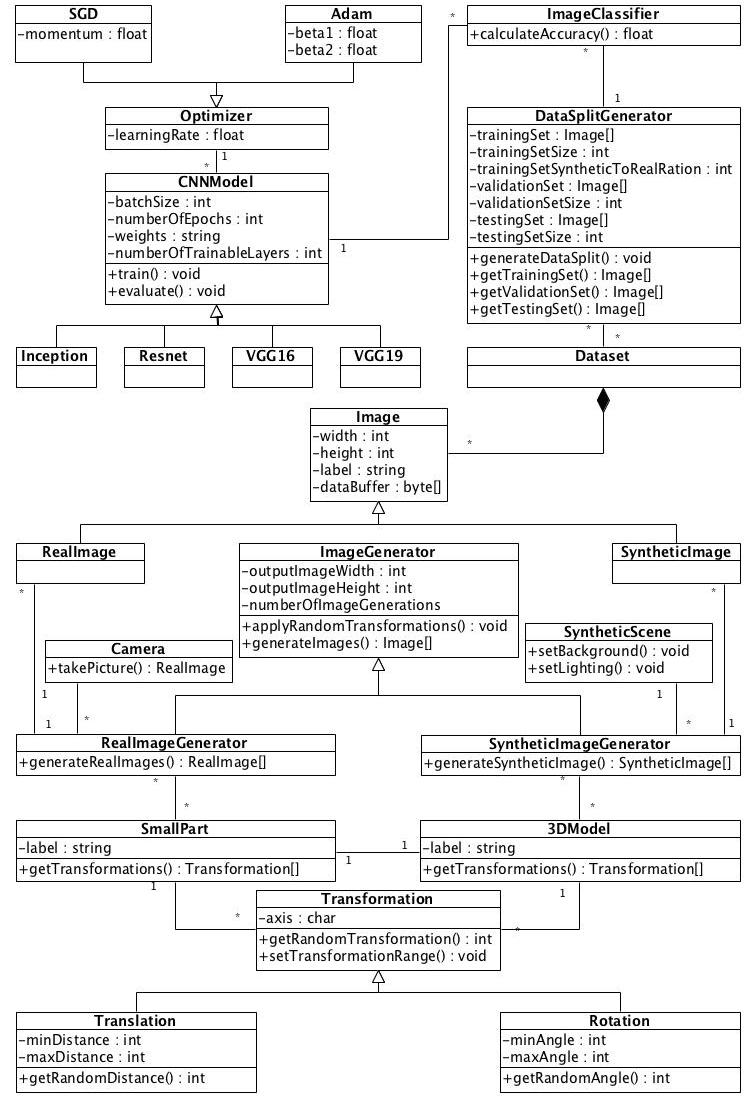
\includegraphics[width=\textwidth]{AOM}
\caption{Analysis Object Model}
\label{fig:AOM}
\end{figure}

\subsection{Dynamic Model}

The dynamic model is focused on the behavior of the system. Sequence diagrams, activity diagrams and state machines are usually used to depict dynamic models \cite{bruegge2004object}. In this section we present 2 activity diagrams that depict the 2 main workflows of our system.

\subsubsection{Dataset Generation}

Figure [\ref{fig:AD1}] depicts the workflow of activities required to generate a dataset. The DataGenerator selects a small part and its corresponding 3D model. The DataGenerator then proceeds to generate the real and synthetic images. Finally the images are combined to form a dataset.

\begin{figure}[H]
\centering
  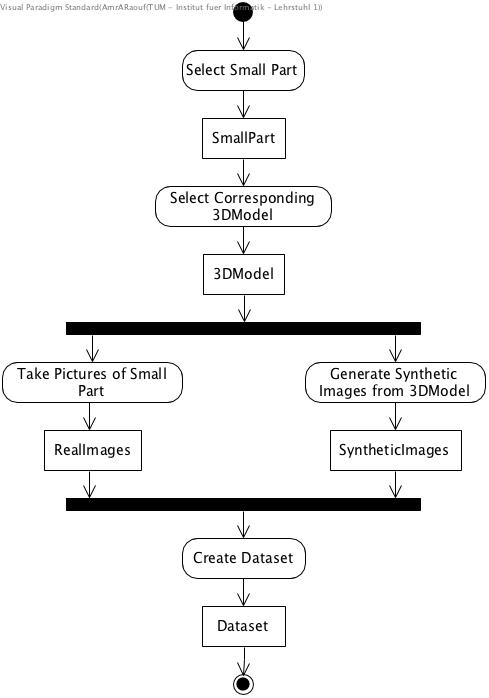
\includegraphics[width=0.65\textwidth]{AD1}
\caption{Activity Diagram depicting the workflow required for Dataset generation}
\label{fig:AD1}
\end{figure}

\subsubsection{Training the Image Classifier}

Figure [\ref{fig:AD2}] describes the workflow of activities required to train the image classifier. The MachineLearningEngineer splits the data into training, validation and testing sets. The MachineLearningEngineer then creates a CNN model. Next the MachineLearningEngineer feeds the training data to the CNN model to obtained a trained CNN model. The MachineLearningEngineer then evaluates the trained CNN model accuracy using the testing set. If the accuracy of the trained CNN model is not sufficient, the CNN model is fine tuned and re-trained.

\begin{figure}[H]
\centering
  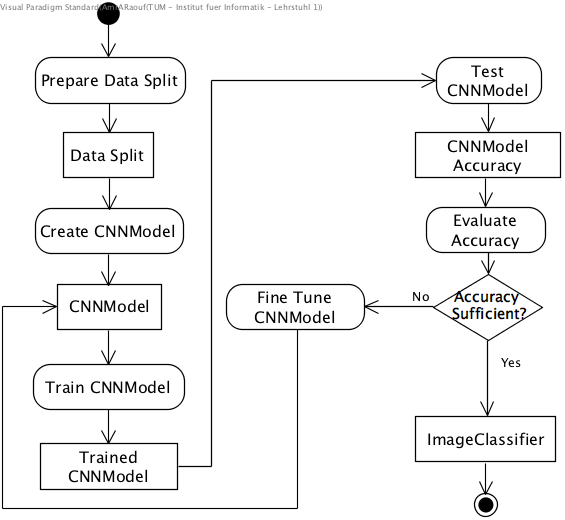
\includegraphics[width=0.7\textwidth]{AD2}
\caption{Activity Diagram describing the workflow required to train the Image Classifier}
\label{fig:AD2}
\end{figure}
